\subsection{Flip-Flop}

\subsubsection{FF SR con porte NAND tipo latch}

In questa prima parte dell'esperienza abbiamo construito il FF SR utilizzando delle porte NAND. Il circuito è riportato in Figura \ref e, come gli altri circuiti logici, il funzionamento è stato verificato con la basetta a LED.

Analizziamo ora il circuito logico. U1 e U2 sono delle porte NAND le cui entrate sono allo stesso potenziale, dunque sono due NOT rispettivamente per i segnali S ed R (terza e quarta colonna della tabella sottostante).

Ad esempio, poniamo ad S ed R l'1 logico: quindi U1 e U2 li renderanno degli 0 logici; dunque, considerando U3 ed U4 come interruttori, se hanno uno degli ingressi a 0 l'uscita sarà sempre 1 indipendentemente dall'altra entrata. Questo stato è poco interessante dal punto di vista logico (non ho due uscite una la negazione dell'altra), quindi cercheremo di evitarlo.

Se invece pongo entrambi gli ingressi di U3 e U4 ad 1 logico (cioè con S=R=0 logico), questi mi restituiranno 1 se l'altro ingresso sarà 0, altrimenti 1. Ciò ovviamente rende le uscite dipendenti dalle tensioni presenti prima del cambiamento di S e di R, rendendolo indeterminate (nel senso che, se non sapessimo i valori di $Q$ e $\bar Q$, a priori non potremmo stabilire, ponendo S=R=0, quale sarà l'uscita). Sfrutteremo questa indeterminazione come elemento di memoria per conservare la nostra informazione fino alla scrittura successiva, che può essere effettuata ponendo S ed R a valori l'uno la negazione dell'altro.

La tabella di verità del circuito logico è la seguente, con $Q_n$ la tensione ad un ciclo e $Q_{n+1}$ quella al ciclo successivo\footnote{In realtà per poter parlare di un ciclo dovremmo attendere la presenza di un attivatore, che se posto come onda quadra ad una certa frequenza può fornirci un clock. Ciò sarà presente nel circuito successivo.}.

\begin{savenotes}
\begin{figure}[H]
		\centering
		{\renewcommand{\arraystretch}{1.1}%
		\begin{tabular}{|c|c|c|c|c|c|}
		\hline
		S & R & $\bar S$ & $\bar R$ & $Q_{n+1}$ & $\bar Q_{n+1}$ \\
		\hline \hline
		0 & 0 & 1 & 1 & $Q_n$ & $\bar Q_n$\\
		\hline
		0 & 1 & 1 & 0 & 0 &1\\
		\hline
		1 & 0 & 0 & 1& 1 & 0\\
		\hline
		1 & 1 &0 &0 & "1" & ”1"\footnote{Ovviamente in questo caso i valori ricavati non rispettano la condizione di essere uno la negazione dell'altro. Abbiamo però voluto inserirli in tabella per sottolineare che questi valori possono essere ricavati, ma sono poco utili per la logica digitale.}\\
		\hline
		\end{tabular}}
		\label{tab11:FFSR}
        \end{figure}
        		\end{savenotes}


Per verificarne il funzionamento, abbiamo collegato entrambe le uscite del Flip-Flop alla basetta al led. Abbiamo notato che non avevamo mai due led accessi contemporaneamente, eccetto nel caso in cui sia Set che Reset erano ad 1 logico, confermando la correttezza della nostra analisi circuitale.

\subsubsection{FF SR con Clock}

In questo secondo circuito vogliamo rendere sincrono quello precedente, inserendo un attivatore (CLK nella tabella sottostante) che possa bloccare eventuali cambiamenti in uscita (cioè la porti in modalità di memoria) indipendentemente da S ed R, come nel circuito in Figura \ref{}. Portando come segnale dell'attivatore una forma d'onda quadra potremmo anche creare un clock. La tabella di verità può essere ricavata con considerazioni analoghe al paragrafo precedente, ed è quella sottostante

\begin{figure}[H]
		\centering
		{\renewcommand{\arraystretch}{1.1}%
		\begin{tabular}{|c||c|c|c|c|}
		\hline
		CLK & S & R & $Q_{n+1}$ & $\bar Q_{n+1}$  \\
		\hline \hline
		0 & X & X & $Q_n$ & $\bar Q_n$\\
		\hline \hline
		 1&0 & 0 & $Q_n$ & $\bar Q_n$\\
		\hline
		1&0 & 1 & 0 &1\\
		\hline
		1&1 & 0 & 1 & 0\\
		\hline
		1&1 & 1 & "1" & "1"\\
		\hline
		\end{tabular}}
		\label{tab11:FFSR2}
        \end{figure}

Notiamo inoltre che anche in questo caso, se sia S che R sono ad 1 logico, le uscite non sono utili per un utilizzo in circuiti logici.

\subsubsection*{Latch tipo D}

Cerchiamo ora di risolvere il problema della presenza dello stato indesiderato dato da S=R=0 logico. Un modo semplice per evitare che possa accadere è di utilizzare il circuito in Figura \ref{}, la cui tabella di verità è la seguente

\begin{figure}[H]
		\centering
		{\renewcommand{\arraystretch}{1.1}%
		\begin{tabular}{|c|c|c|c|}
		\hline
		D & CLK & $Q_{n+1}$ & $\bar Q_{n+1}$  \\
		\hline
		X & 0  & $Q_n$ & $\bar Q_n$\\
		\hline
		 1&1 & 1 & 0\\
		\hline
		0&1 & 0  &1\\
		\hline
		\end{tabular}}
		\label{tab11:Latch_D}
        \end{figure}

Abbiamo inoltre notato che, con CLK ad 1, lasciando l'ingresso D flottante l'uscita Q era bassa. Ciò è in contraddizione con le porte integrate, in quanto quando un ingresso non è collegato a nessun riferimento viene visto come alto. Abbiamo capito che ciò era dovuto al fatto che abbiamo collegato il cavo dati alla basetta al led per vedere quando esso era a 0 o 1 logico. La basetta al led è costruita con resistenze di pull-down così che quando il segnale in ingresso è basso i led sono spenti. Dunque se monitoriamo il segnale D con la basetta, esso è collegato con resistenze di pull-down a comune. Abbiamo infatti verificato che scollegandolo dalla basetta, l'ingresso D flottante causava un uscita Q alta.

\subsubsection*{Circuito anti-rimbalzo}


\begin{wrapfigure}[14]{l}{0.45\textwidth}
\centering
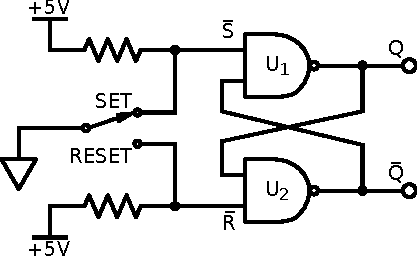
\includegraphics[width=.25\textwidth]{../E11/latex/anti-rimbalzo.pdf}
\caption{.}
\label{cir11:no-rimb}
\end{wrapfigure}

Un problema degli interruttori è quello del rimbalzo. Infatti lo switch meccanico dell'interruttore non è istantaneo in quanto composto da una linguetta conduttrice che fa da contatto. Nel momento in cui la linguetta passa da un contatto all'altro abbiamo dei rimbalzi di tensione. Un modo per risolvere questo problema è quello di utilizzare un interruttore a transistor oppure inserire appena dopo l'interruttore meccanico un circuito di anti-rimbalzo. Lo schema è riportato in figura (\ref{cir11:no-rimb}). Tale circuito ci permette di evitare i rimbalzi poichè quando la linguetta è scollegata sia dal SET che dal RESET abbiamo il circuito in configurazione memoria. Ciò è dovuto al fatto che abbiamo inserito delle resistenze di Pull-Up che portano gli ingressi delle NAND a 1 logico. 

Di seguito è riportata la tabella di verità del circuito.




\begin{figure}[H]
		\centering
		{\renewcommand{\arraystretch}{1.1}%
		\begin{tabular}{c|c|c|c}
		$\bar S$ & $\bar R$ & $Q_{n+1}$ & $\bar Q_{n+1}$  \\
		\hline
		0 & 0  & ?&?\\
		\hline
		0&1 & 1 & 0\\
		\hline
		1&0 & 0  &1\\
		\hline
		1&1 & $Q_n$ & $\bar Q_n$\\
		\end{tabular}}
		\label{tab11:antirimb}
		\caption{puzzi ancora di più di buzz}
        \end{figure}


Dopo averne studiato le caratteristiche dal punto di vista teorico, ne abbiamo verificato il funzionamento sperimentalmente. I risultati sono riportati nei seguenti grafici.


$$**grafici**$$


Come vediamo, il tempo di rimbalzo senza correzione è di circa \SI{4}{\milli\second}. Utilizzando il circuito FF, invece, abbiamo completamente eliminato il problema. La forma d'onda in uscita non è perfettamente a scalino in quanto i generatori di corrente non sono ideali e le impedenze non sono ottimizzate. 


\subsection*{Comandi separati Marcia/Arresto}

Possiamo apportare delle utili modifiche al circuito anti-rimbalzo separando il comando Marcia/Arresto. Così facendo possiamo avere un circuito che può essere messo nella condizione di memoria. Il circuito è riportato in fugura (\ref{cir11:marcia}).

\begin{figure}[H]
\centering
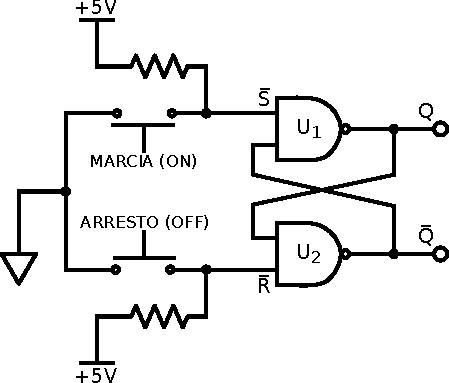
\includegraphics[width=.25\textwidth]{../E11/latex/motorefermo.pdf}
\caption{.}
\label{cir11:marcia}
\end{figure}

Dobbiamo ricordarci di non mettere mai contemporaneamente a 0 logico sia Marcia che Arresto in quanto avremmo una condizione di indeterminazione che ovviamente non vogliamo.


\subsubsection*{FF SR con porte NOR}

Abbiamo provato a realizzare un FF SR con porte NOR. Il principio di funzionamento è lo stesso di quello costruito utilizzando porte NAND. L'unica differenza sta nel fatto che il circuito si trova in memoria quando sia S che R sono a 0 logico. Lo schema circuitale elaborato è riportato nella seguente figura.

\begin{figure}[H]
\centering
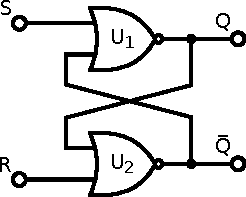
\includegraphics[width=.25\textwidth]{../E11/latex/FF-w-NOR.pdf}
\caption{.}
\label{cir11:nor}
\end{figure}

Per completezza riportiamo anche la tabella di verità del circuito. Il circuito, come sempre, è stato verificato utilizzado la basetta a led.

\begin{figure}[H]
		\centering
		{\renewcommand{\arraystretch}{1.1}%
		\begin{tabular}{c|c|c|c}
		S & R & $Q_{n+1}$ & $\bar Q_{n+1}$  \\
		\hline
		1 & 1  & ?&?\\
		\hline
		1&0 & 1 & 0\\
		\hline
		0&1 & 0  &1\\
		\hline
		0&0 & $Q_n$ & $\bar Q_n$\\
		\end{tabular}}
		\label{tab11:nor}
		\caption{.}
        \end{figure}


\subsubsection*{Divisore di frequenze}

Come ultima parte dell'esperienza abbiamo realizzato un divisore di frequenze. Tale circuito, utilizzando dei FF di tipo T (Toggle), permette di fare una divisione di frequenze per multipli di 2. In effetti, utilizzando un circuito 


